\section{Các phương pháp cải tiến}
\subsection{Sliding Window}
\subsection{Khắc phục vấn đề mất dữ liệu}
\subsection{Cải thiện chất lượng mô hình}
\subsubsection{Mô hình với Deep Convolution và Self-Attention}

Trong đề tài trước, mô hình học máy được sử dụng khá thô sơ và đơn giản, bao gồm các thành phần chính: một lớp \textit{LSTM}, một lớp \textit{Dropout}, một lớp \textit{Flatten}, và hai lớp \textit{Dense}. 

\begin{figure}[H]
    \centering
    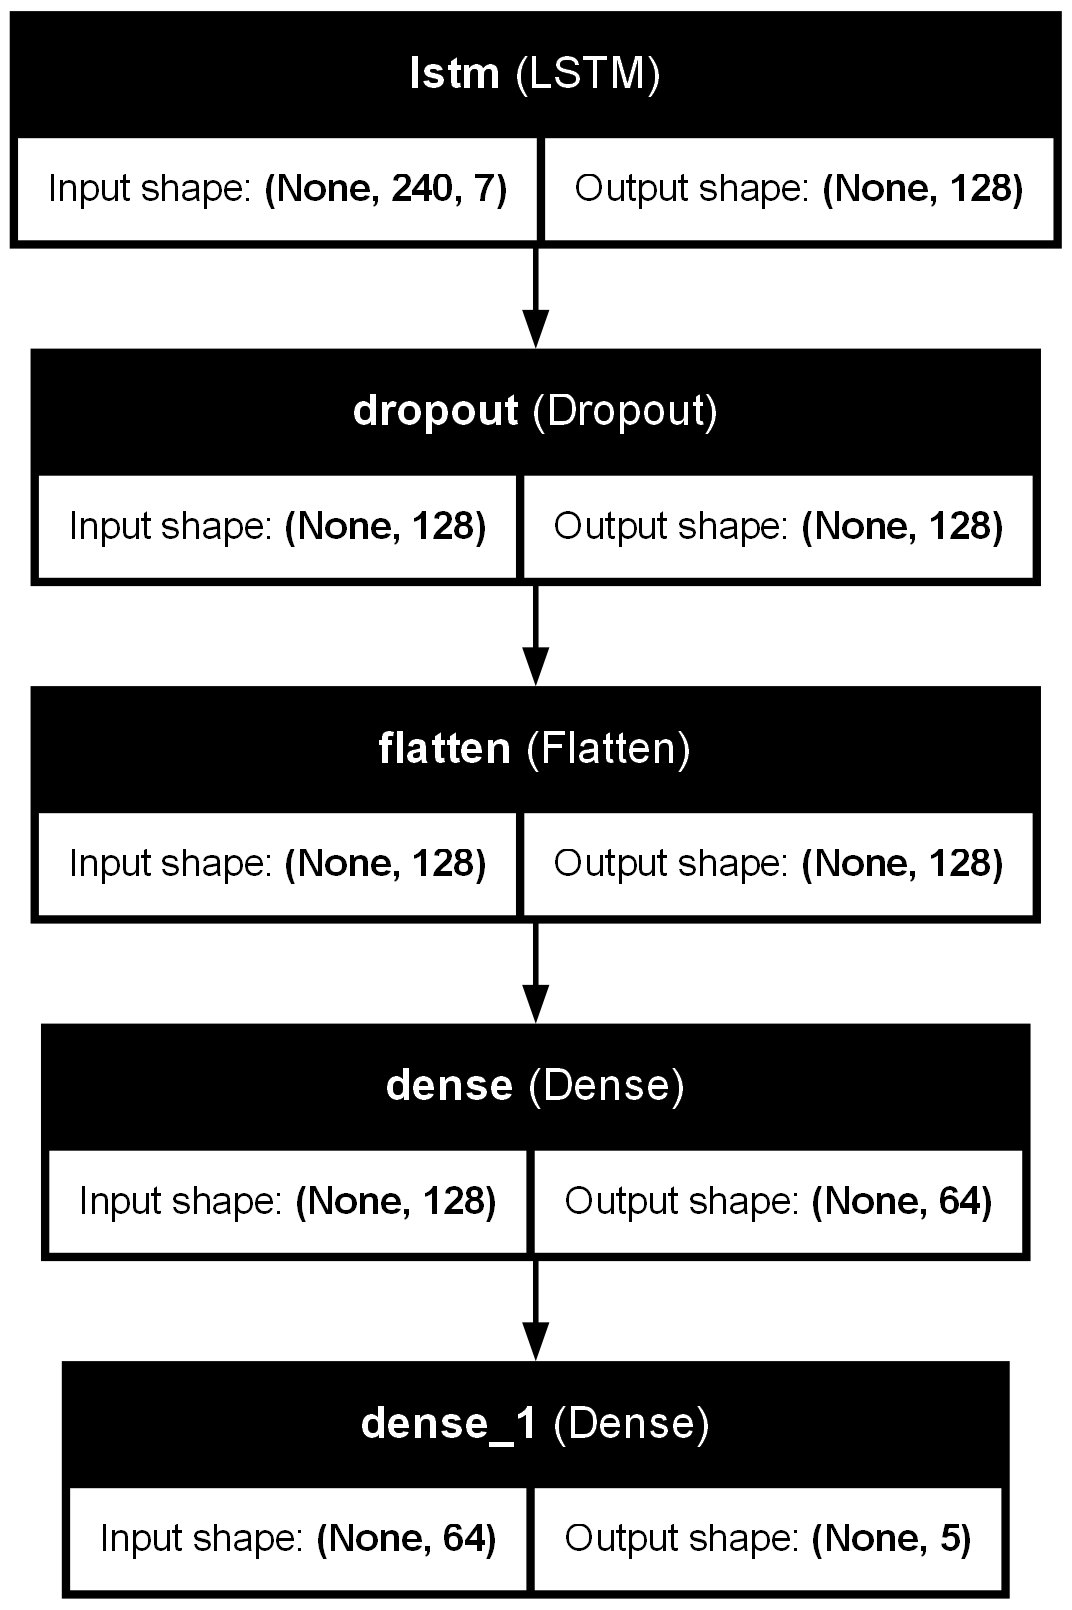
\includegraphics[width=0.5\linewidth]{Images/Improved methods/old_model_plot.png}
    \caption{Cấu trúc mô hình cũ}
    \label{fig:old-model}
\end{figure}

Kết quả đạt được từ mô hình này vẫn chưa thực sự khả quan. Để cải thiện chất lượng đầu ra, cần thực hiện hai bước quan trọng:
\begin{itemize}
    \item \textbf{Gia tăng kích thước tập dữ liệu}: Mở rộng và đa dạng hóa dữ liệu đầu vào.
    \item \textbf{Nâng cấp mô hình}: Sử dụng kiến trúc học máy hiệu quả hơn để khai thác triệt để thông tin từ dữ liệu.
\end{itemize}

Trong đề tài này, nhóm đề xuất một mô hình cải tiến, dựa trên kiến trúc được giới thiệu trong bài báo \textit{"Self-Attention-Based Deep Convolution LSTM Framework for Sensor-Based Badminton Activity Recognition"} (\href{https://doi.org/10.3390/s23208373}{DOI: 10.3390/s23208373}). Mô hình này kết hợp:
\begin{enumerate}
    \item \textbf{Mạng nơ-ron tích chập (CNN)}: Chiết xuất các đặc trưng cục bộ từ dữ liệu đầu vào.
    \item \textbf{Mạng nơ-ron hồi quy (LSTM)}: Nắm bắt các phụ thuộc dài hạn trong dữ liệu.
    \item \textbf{Cơ chế Self-Attention}: Tập trung vào các phần quan trọng nhất của dữ liệu.
\end{enumerate}

Mô hình đề xuất bao gồm các thành phần chính sau:
\begin{itemize}
    \item \textbf{Lớp CNN}: Chiết xuất các đặc trưng cục bộ từ dữ liệu đầu vào.
    \item \textbf{Lớp LSTM}: Nắm bắt và lưu giữ các thông tin phụ thuộc dài hạn trong chuỗi thời gian.
    \item \textbf{Cơ chế Self-Attention}: Xác định và tập trung vào các đặc trưng quan trọng nhất trong dữ liệu, cải thiện hiệu quả học hỏi của mô hình.
\end{itemize}

\begin{figure}[H]
    \centering
    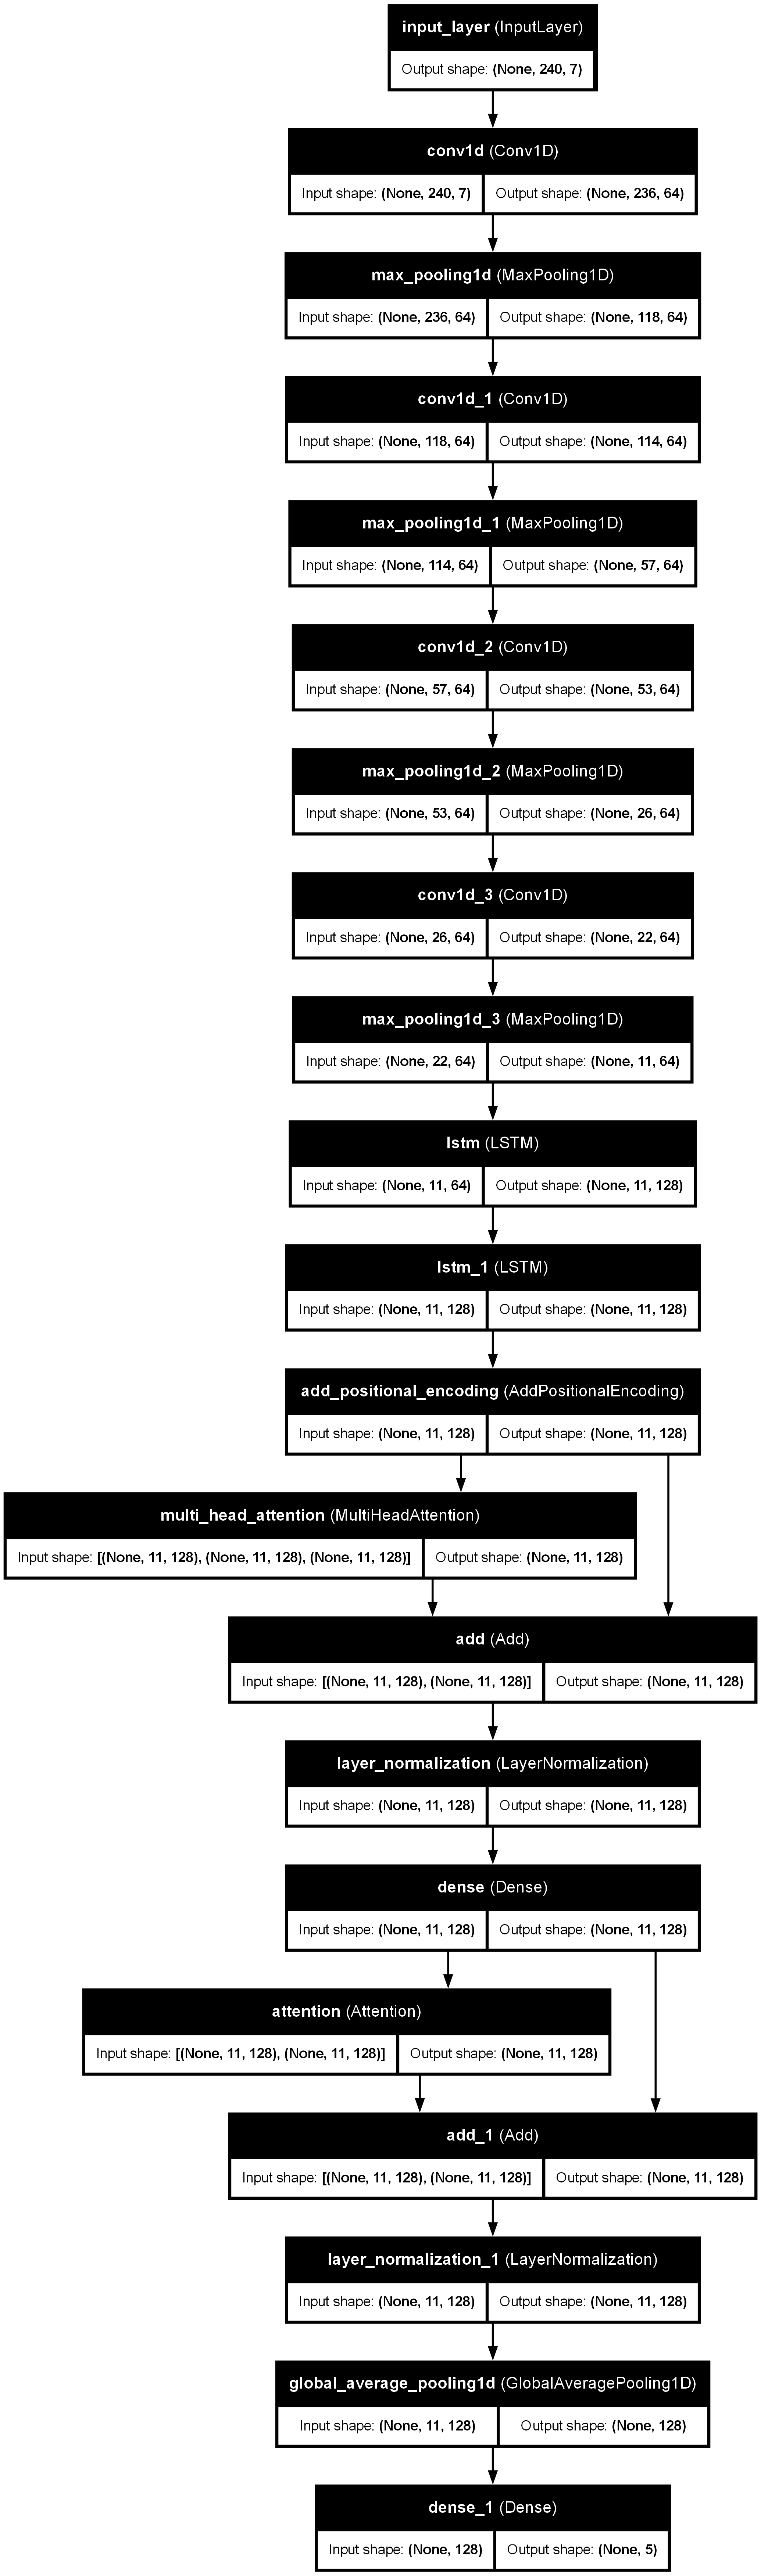
\includegraphics[width=0.4\linewidth]{Images/Improved methods/new_model_plot.png}
    \caption{Mô hình mới}
    \label{fig:new-model}
\end{figure}


\noindent
Cơ chế \textit{Self-Attention} đóng vai trò then chốt trong việc nâng cao hiệu suất của mô hình. Nó cho phép mô hình tự động:
\begin{itemize}
    \item Phân tích toàn bộ dữ liệu đầu vào.
    \item Tập trung vào những đặc trưng mang tính quyết định.
\end{itemize}

Nhờ vậy, mô hình có thể đạt được độ chính xác cao hơn trong việc dự đoán các hành động theo chuỗi thời gian.

\subsection{Làm giàu dữ liệu}
\subsubsection{Data Augmentation}

Trong học máy, \textit{Data Augmentation} là một kỹ thuật quan trọng giúp mở rộng tập dữ liệu hiện có bằng cách tạo ra các biến thể mới của dữ liệu. Điều này không chỉ cải thiện tính đa dạng của dữ liệu mà còn giúp mô hình giảm thiểu hiện tượng quá khớp (\textit{overfitting}) và học được nhiều đặc trưng tổng quát hơn. Dưới đây là một số kỹ thuật được áp dụng:

\begin{enumerate}

\item \textbf{Jittering}: 
\begin{itemize}
\item \textbf{Mô tả}: Thêm nhiễu ngẫu nhiên vào dữ liệu. Jittering có thể được thực hiện bằng cách thêm một lượng nhỏ nhiễu Gaussian vào mỗi điểm dữ liệu. Điều này giúp mô hình ít bị ảnh hưởng bởi nhiễu trong dữ liệu thực tế và tăng khả năng kháng nhiễu của mô hình.
\item \textbf{Lợi ích}: 
\begin{itemize}
\item Giúp mô hình trở nên mạnh mẽ hơn trước các biến động nhỏ trong dữ liệu thực tế.
\item Tăng khả năng tổng quát hóa bằng cách làm cho dữ liệu đầu vào đa dạng hơn.
\end{itemize}
\end{itemize}

\item \textbf{Scale}: 
\begin{itemize}
\item \textbf{Mô tả}: Thay đổi tỷ lệ của dữ liệu. Scale được thực hiện bằng cách nhân mỗi điểm dữ liệu với một hệ số tỷ lệ ngẫu nhiên.
 \item \textbf{Lợi ích}:
\begin{itemize}
\item Giúp mô hình học được các đặc trưng ở các mức độ hoặc tỉ lệ khác nhau.
 \item Phù hợp với các bài toán mà dữ liệu có sự biến thiên về kích thước, chẳng hạn như tín hiệu sinh lý.
\end{itemize}
 \end{itemize}

\item \textbf{Magnitude Warp}: 
\begin{itemize}
\item \textbf{Mô tả}: Biến dạng biên độ của dữ liệu theo một hàm phi tuyến. Magnitude Warp có thể được thực hiện bằng cách áp dụng một hàm phi tuyến, chẳng hạn như hàm sin hoặc hàm mũ, cho biên độ của dữ liệu.
\item \textbf{Lợi ích}:
\begin{itemize}
\item Tạo ra các biến thể tín hiệu thực tế hơn, đặc biệt phù hợp với các bài toán liên quan đến chuỗi thời gian.
\item Làm phong phú tập dữ liệu và giúp mô hình ít phụ thuộc vào các dạng tín hiệu cụ thể.
 \end{itemize}
\end{itemize}

\item \textbf{Shift}: 
 \begin{itemize}
 \item \textbf{Mô tả}: Dịch chuyển dữ liệu theo thời gian. Shift được thực hiện bằng cách dịch chuyển toàn bộ chuỗi thời gian sang trái hoặc phải một khoảng thời gian ngẫu nhiên.
 \item \textbf{Lợi ích}:
\begin{itemize}
\item Tăng khả năng chống lại sự thay đổi vị trí trong dữ liệu, chẳng hạn như các tín hiệu không đồng bộ.
\item Giúp mô hình học được các đặc trưng không bị phụ thuộc vào vị trí cụ thể.
\end{itemize}
\end{itemize}

\end{enumerate}

Để tăng cường dữ liệu huấn luyện, nhóm đã xây dựng một script Python để áp dụng các kỹ thuật Data Augmentation đã đề cập ở trên. Script này nhận dữ liệu gốc làm đầu vào và tạo ra các phiên bản biến đổi của dữ liệu bằng cách sử dụng các kỹ thuật Jittering, Scale, Magnitude Warp và Shift.

Mỗi kỹ thuật Data Augmentation được áp dụng riêng biệt, tạo ra một phiên bản mới của tập dữ liệu với cùng kích thước với tập dữ liệu gốc. Do đó, sau khi áp dụng cả bốn kỹ thuật, nhóm thu được một tập dữ liệu mới có kích thước gấp 5 lần tập dữ liệu ban đầu (bao gồm cả dữ liệu gốc). 

Việc tăng kích thước tập dữ liệu huấn luyện thông qua Data Augmentation giúp cải thiện khả năng tổng quát hóa của mô hình, giảm thiểu hiện tượng overfitting và tăng cường độ chính xác của mô hình trên dữ liệu mới.
\subsubsection{Transfer learning}
Một cách cải thiện hiệu suất của mô hình là sử dụng \textit{Transfer learning}. Transfer learning là một kỹ thuật học máy mà mô hình được huấn luyện trước trên một tập dữ liệu lớn và sau đó được sử dụng để giải quyết một bài toán mới. Nhóm sử dụng một tập dữ liệu có tên là "DU-ASL-DATA-GLOVE-DB" được công bố trên trang web \href{https://figshare.com/articles/dataset/ASL-Sensor-Dataglove-Dataset_zip/20031017?file=35776586}{Figshare}. Tập dữ liệu này chứa dữ liệu về ngôn ngữ ký hiệu Mỹ (ASL) được thu thập từ cảm biến găng tay thông minh.

\begin{itemize}
    \item \textbf{Tổng quan:} Đây là một tập dữ liệu được thu thập bởi 1 nhóm sinh viên chuyên ngành kỹ thuật sinh học tại Ấn Độ, họ thu thập dữ liệu từ 25 người khác nhau (19 nam và 6 nữ). Mỗi người thực hiện 40 cử chỉ khác nhau (26 cử chỉ trong bảng chữ cái và 14 từ). Dữ liệu được thu thập từ cảm biến với tần số lấy mẫu 100Hz và mỗi cử chỉ có thời lượng 1.5 giây và được thực hiện 10 lần cho mỗi đối tượng.
    \item \textbf{Thông tin phần cứng:} Dữ liệu được thu thập từ 5 cảm biến flex 2.2 inch SEN-10264 và 1 cảm biến IMU MPU6050.
    \item \textbf{Tổ chức dữ liệu:} Dữ liệu được lưu trong 25 thư mục được đánh số từ 001 đến 025, mỗi thư mục chứa dữ liệu của một người. Mỗi thư mục chứa 40 file csv tương ứng với 40 cử chỉ khác nhau. Mỗi file csv chứa dữ liệu của 10 lần thực hiện cử chỉ. 
    \item \textbf{Tiền xử lý:} Dữ liệu cần được xử lý để có thể phu hợp với mô hình của nhóm. Mô hình học máy nhóm sử dụng yêu cầu dữ liệu đầu vào phải có timestep là 250 và số chiều là 7. Do đó nhóm cần thực hiện 2 bước tiền xử lý chính:
    \begin{itemize}
        \item \textbf{Thay đổi tập dữ liệu} Vì tín hiệu ở cột thứ 4 được tính bằng tổng tín hiệu của cảm biến từ ngón áp út và ngón út, nhóm cần phải tính lại giá trị của cột này bằng cách tính tổng điện trở của f4 và f5 trong dataset. Nhóm cũng chỉ sử dụng giá trị từ flex sensor và cảm biến góc quay vì thiết bị không có cảm biến gia tốc.
        \item \textbf{Upscaling dữ liệu:} Dữ liệu được thu thập với tần số lấy mẫu 100Hz với thời gian thực hiện cử chỉ là 1.5 giây. Điều đó có nghĩa là dữ liệu thu được có số lượng timestep là 150. Để phù hợp với mô hình nhóm sử dụng, nhóm cần phải upscaling dữ liệu lên 250 timestep. Kỹ thuật upscaling được sử dụng là nội suy tuyến tính.
    \end{itemize}
    \begin{figure}
        \centering
        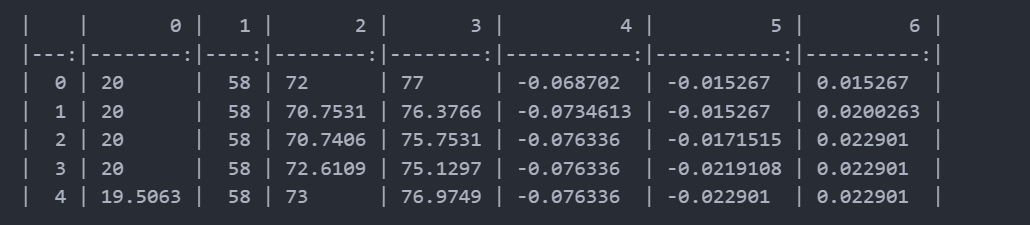
\includegraphics[width=0.8\linewidth]{Images/Improved methods/transfer_learning.png}
        \caption{Dữ liệu sau khi chỉnh sửa}
        \label{fig:interpolation}
    \end{figure}
    \item \textbf{Huấn luyện mô hình:} Mô hình được sử dụng là mô hình cải tiến mà nhóm đã giới thiệu ở trên. Mô hình được huấn luyện trên tập dữ liệu ASL. Weight của mô hình được lưu lại và sử dụng cho việc huấn luyện mô hình trên tập dữ liệu của nhóm.
\end{itemize}
\subsubsection{Sinh dữ liệu từ TimeGAN}
